
\section{Introduction}\index{Introduction}

The purpose of a particle physics detector is find all the particles produced
in a collision, identify which type of particle each is, and measure its 4-momenta.
At the LHC, in a single collision, thousands of particles can be produced.
The particle physics detector must make signals that somehow can yield this information.
To understand how this can happen, we first must understand how particles interact
with matter, so we can learn of the possible types of signals particles could produce.

What kinds of particles can an LHC detector detect?  First, the particle must live long 
enough to reach the detector, without decaying.  The beam pipe of the LHC has a 
radius with dimensions measured in cm.  The particle must exist the beam pipe to
reach the detector and make a signal.  If we take the diameter to be 1 cm, then
the particle life time must be large enough to travel this far before decay.

The particle must also interact strongly enough with matter to produce a signal in a detector that is small enough to be affordable.  While specialized very large detectors exist which can detect neutrinos, this is not possible at a collider detector.

There are only a few types of particles (and their antiparticles) that satisfy these requirements, and they are:
\begin{itemize}
\item from the leptons
\begin{itemize}
\item electrons
\item muons
\end{itemize}
\item from the bosons
\begin{itemize}
\item photons
\end{itemize}
\item from the mesons
\begin{itemize}
\item charged pions
\item k-longs (a very rare particle)
\end{itemize}
\item from the baryons
\begin{itemize}
\item protons
\item neutrons
\end{itemize}
\end{itemize}

The most common particle produced in a proton-proton collision is the pion.  Neutral pions decay very quickly to two photons. Most of the particles we detect, therefore, will be charged pions and photons.  However, as we will discuss, particles like electrons and muons are signatures of Higgs decays, and so we need to have a detector well optimized for identifying and measuring these particles as well.




\section{Interactions of charged particles with matter}\index{chargedinteractions}
We will first look at possible signals from charged particles (electrons, muons, charged pions, protons).

Possible interactions between these particles and bulk matter include:
\begin{itemize}
\item ionizaiton and excitation of the molecules in the material
\item bremsstrahlung
\item nuclear interactions (for the particles that interact via the strong force because they contain quarks, the pions and protons)
\end{itemize}
We will postphone the discussion of the later two until our discussion of ``calorimetry'' and discuss only the first in this chapter.

When a charged particle passes through some material (detectors are often made of Argon gas, silicon, iron, lead, steel, plastic, and other such materials), it will interact with the electrons in the molecules that make up that material via the electric force.  The charged particle loses energy as it passes through the material, and the material gains energy.  What effect does that energy have on the material?  It can cause the electrons in the material to ``be excited'' into higher quantum states or it can even detach an electron from its atom (``ionization'').  

One important parameter regarding this energy lose is called $dE/dx$, pronounced ``d-E-d-x''.  $dE/dx$ is the amount of energy lost by the particle per unit length transversed.  The average amount of energy lost per unit length depends on the energy of the particle: low energy particles lose more energy per unit length than high energy particles.  You can imagine why this might be true: the lower energy (slower) particles linger near each atom in the material longer, and thus have a longer time to interact with each one and lose more energy.

Figure ~\ref{fig:pdgdedx} shows the energy dependence of dedx for muons.  Note that the length unit is strange: it is $cm^2/g$.  You can convert this to length by multiplying by the density of the material
\begin{equation}
{{MeV cm^2}\over{g}} \cdot {{g}\over{cm^3}} = {{MeV}\over{cm}}
\end{equation}

\begin{figure}[h]
\centering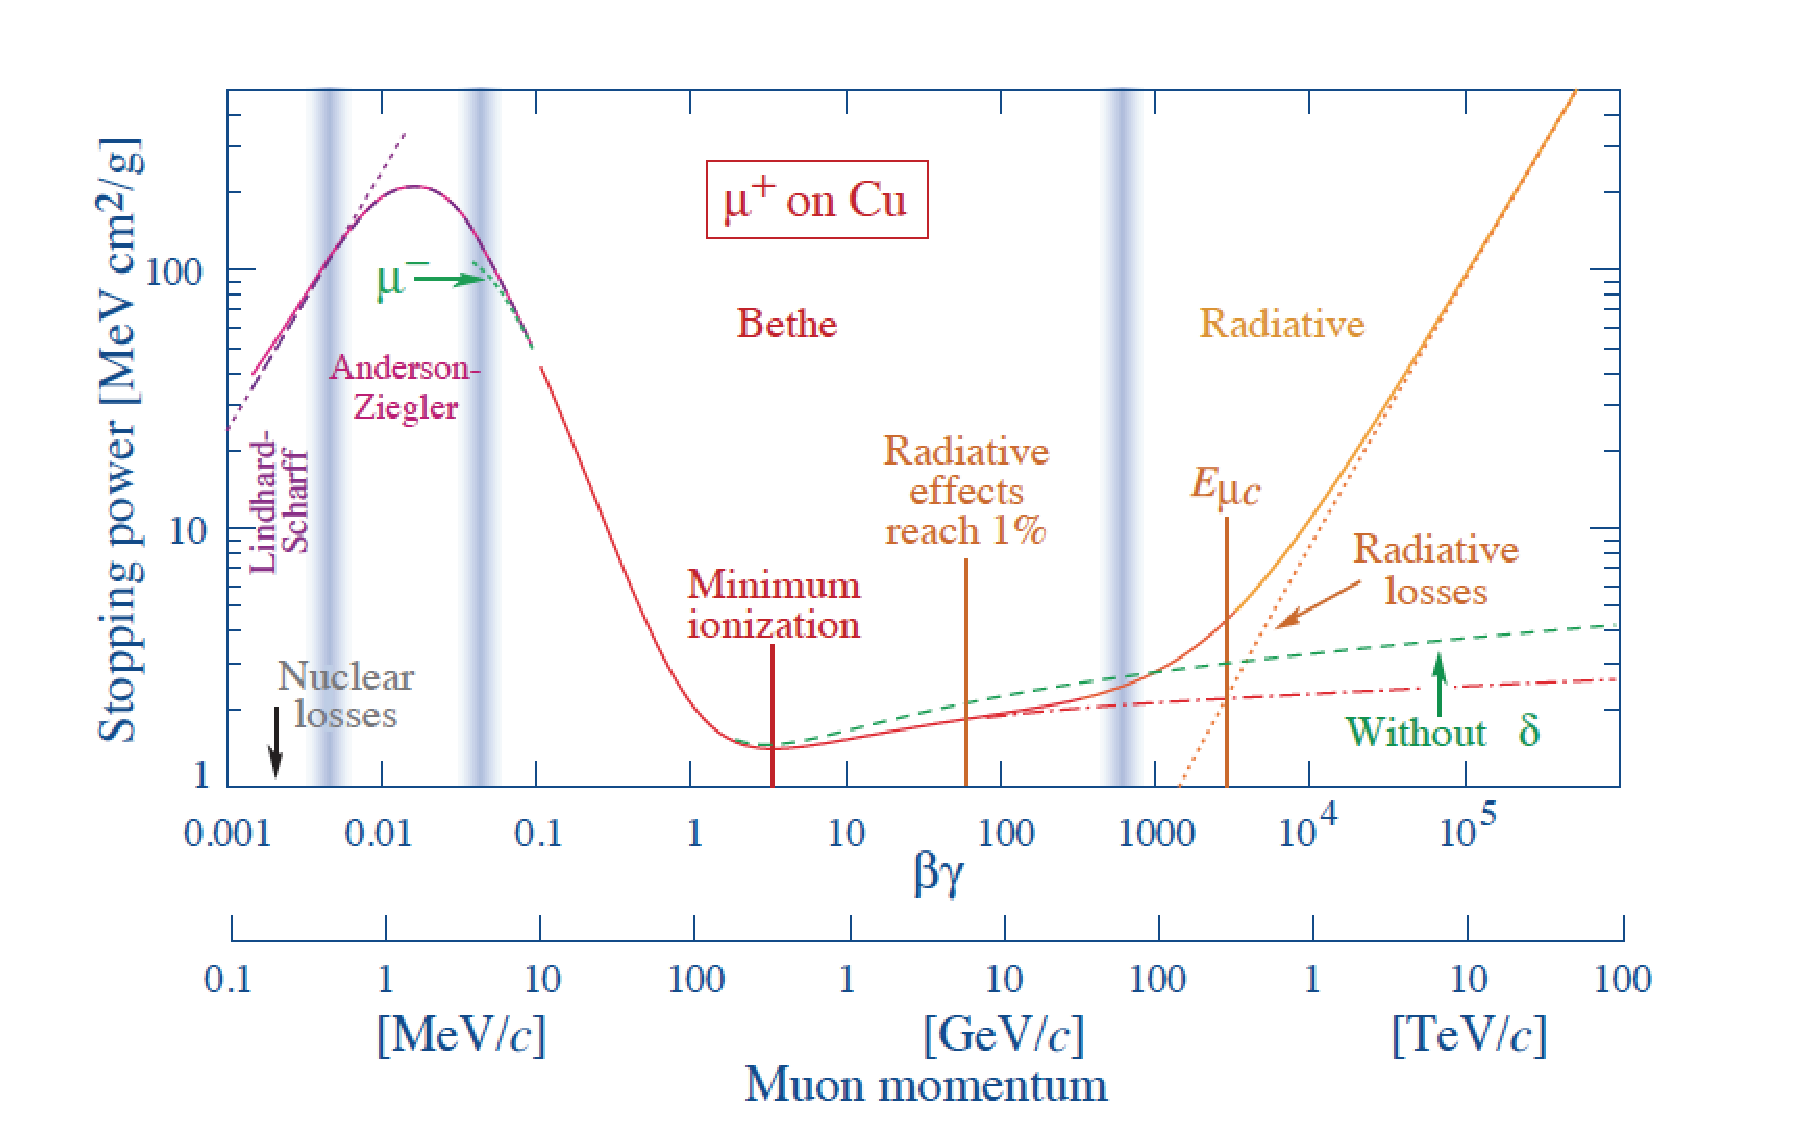
\includegraphics[scale=0.5]{./particleinteractions/Pictures/dedx.eps}
\caption{Stolen from the particle data group, this picture shows the energy
loss per unit length as a function of particle energy for muons}
\label{fig:pdgdedx}
\end{figure}

What kind of signals can be produced this way?  If the material is a gas, the electrons produced through ionization can be gathered on a wire (using an electric field produced by voltages on metal pads on the structure holding the gas or on wires running through the gas) to produce a current.  The signals from silicon are similar.  If the material is a plastic scintilator, some of the ``excited'' molecules will ``de-excite'' by emitting photons, which can be detected with a photomulitplier tube or other light sensitive device.

If the material is thick and high-Z (iron, lead), the particle may lose all its energy and 
stop inside the material.  The thickness of material that will stop a particle (of a given energy) is called the particle's range.


\section{Interactions of gamma rays with matter}\index{gammainteractions}

Here we call them “gamma rays” instead of photons because we are going to discuss only those photons of interest to particle physics: ones with energies above a keV or so.

There are several ways a gamma ray can interaction with matter:
\begin{itemize}
\item photoelectric effect
\end{itemize}

The most important of these is pair production.  We will discuss this more when we discuss calorimetry.

